%%%%%%%%%%%%%%%%%%%%%%%%%%%%%%
%
% $Autor: Wings $
% $Datum: 2019-12-09 11:50:02Z $
% $Pfad: komponenten/Bilderkennung/Produktspezifikation/CorelTPU/TPU/Allgemein/tikzdefs.tex $
% $Version: 1766 $
%
%
%%%%%%%%%%%%%%%%%%%%%%%%%%%%%%


% Definition für tikz

\usepackage{pgfplots}
\usepackage{pgf,tikz}
\usepackage{mathrsfs}
\usepackage{tikz}
\usetikzlibrary{shapes,shapes.symbols,shapes.misc, shapes.multipart, shapes.geometric,arrows,angles,quotes,babel,positioning,calc,math,matrix,backgrounds}
\usetikzlibrary{positioning,fadings,through}


\usepackage{tikz-3dplot}

\tikzset{
  input2/.style={ % requires library shapes.geometric
    draw,
    trapezium,
    trapezium left angle=60,
    trapezium right angle=120,
  },
  process rectangle outer width/.initial=0.15cm,
  predefined process/.style={
    rectangle,
    draw,
    append after command={
      \pgfextra{
        \draw [fill=blue!20]
        ($(\tikzlastnode.north west)-(0,0.5\pgflinewidth)$)--
        ($(\tikzlastnode.north west)-(\pgfkeysvalueof{/tikz/process rectangle outer width},0.5\pgflinewidth)$)--
        ($(\tikzlastnode.south west)+(-\pgfkeysvalueof{/tikz/process rectangle outer width},+0.5\pgflinewidth)$)--
        ($(\tikzlastnode.south west)+(0,0.5\pgflinewidth)$);
        \draw [fill=blue!20]
        ($(\tikzlastnode.north east)-(0,0.5\pgflinewidth)$)--
        ($(\tikzlastnode.north east)+(\pgfkeysvalueof{/tikz/process rectangle outer width},-0.5\pgflinewidth)$)--
        ($(\tikzlastnode.south east)+(\pgfkeysvalueof{/tikz/process rectangle outer width},0.5\pgflinewidth)$)--
        ($(\tikzlastnode.south east)+(0,0.5\pgflinewidth)$);
      }  
    },
    text width=#1,
    align=center, fill=blue!20,  minimum height=4em
  },
  predefined process/.default=20mm,
  data1/.style={
    trapezium, 
    trapezium left angle=70, 
    trapezium right angle=110, 
    text width=1.5cm, 
    inner ysep=17pt,
    align=center, 
    line width=2pt,
    fill=blue!20
  },      
}


%Kabinettprojektion von 3D auf 2D
%
% Eingabe
% x,y,z
%
% Ausgabe
% x- oder y-Wert des Punkts
\newcommand{\Proj}[3]{({#1-#3*0.5*cos(30)},{#2-#3*0.5*sin(30)})}
\tikzset{declare function={ProjX(\x,\y,\z)=\x-\z*0.5*cos(30);}}
\tikzset{declare function={ProjY(\x,\y,\z)=\y-\z*0.5*sin(30);}}

%Rotation um die x-Achse 
%
% Eingabe
% x,y,z,alpha
%
% Ausgabe
% 
% x-, y- oder z-Wert des Punkts
\tikzset{declare function={RotXx(\x,\y,\z,\a)=\x;}}
\tikzset{declare function={RotXy(\x,\y,\z,\a)=\y*cos(\a)-\z*sin(\a);}}
\tikzset{declare function={RotXz(\x,\y,\z,\a)=\y*sin(\a)+\z*cos(\a);}}


%Rotation um die y-Achse 
%
% Eingabe
% x,y,z,alpha
%
% Ausgabe
% 
% x-, y- oder z-Wert des Punkts
\tikzset{declare function={RotYx(\x,\y,\z,\a)=\x*cos(\a)-\z*sin(\a);}}
\tikzset{declare function={RotYy(\x,\y,\z,\a)=\y;}}
\tikzset{declare function={RotYz(\x,\y,\z,\a)=\x*sin(\a)+\z*cos(\a);}}



%Rotation um die z-Achse 
%
% Eingabe
% x,y,z,alpha
%
% Ausgabe
% 
% x-, y- oder z-Wert des Punkts
\tikzset{declare function={RotZx(\x,\y,\z,\a)=\x*cos(\a)-\y*sin(\a);}}
\tikzset{declare function={RotZy(\x,\y,\z,\a)=\x*sin(\a)+\y*cos(\a);}}
\tikzset{declare function={RotZz(\x,\y,\z,\a)=\z;}}


%Rotation um die x-Achse 
%
% Eingabe
% x,y,z,alpha
%
% Ausgabe
% Punkt {x}{y}{z}
\newcommand{\RotXx}[4]{#1}%
\newcommand{\RotXy}[4]{(cos(#4)*#2-sin(#4)*#3)}
\newcommand{\RotXz}[4]{(sin(#4)*#2+cos(#4)*#3)}%


\tikzset{declare function={bellshape(\x,\mu,\sigma)=exp(-(\x-\mu)^2/(2*\sigma^2));}}


%Rotation um die x-Achse mit Projektion
%
% Eingabe
% x,y,z,alpha
%
% Ausgabe
% Punkt ({x}, {y})
\newcommand{\RotXP}[4]%
{(%
{#1-(sin(#4)*#2+cos(#4)*#3)*0.5*cos(30)},%
{cos(#4)*#2-sin(#4)*#3-(sin(#4)*#2+cos(#4)*#3)*0.5*sin(30)})%
}

%Rotation um die y-Achse mit Projektion
%
% Eingabe
% x,y,z,alpha
%
% Ausgabe
% Punkt ({x}, {y})
\newcommand{\RotYP}[4]%
{(%
{cos(#4)*#1+sin(#4)*#3-(-sin(#4)*#1+cos(#4)*#3)*0.5*cos(30)},%
{#2-(-sin(#4)*#1+cos(#4)*#3)*0.5*sin(30)}%
)}


%Rotation um die z-Achse mit Projektion
%
% Eingabe
% x,y,z,alpha
%
% Ausgabe
% Punkt ({x}, {y})
\newcommand{\RotZP}[4]%
{({cos(#4)*#1-sin(#4)*#2-#3*0.5*cos(30)},{sin(#4)*#1+cos(#4)*#2-#3*0.5*sin(30)})}


% Parameter
% #1: Skalierung
% #2: Winkel; 0..179
\newcommand{\HermiteSymPSP}[2]{%
  \pgfmathsetmacro{\RADIUS}{6}
  
  \begin{scope}[scale=#1]
    
    % angle 
    \begin{scope}[shift={(\RADIUS,0cm)}]
      \draw[fill=green!30] (0,0) -- (180:0.25*\RADIUS) arc (180:#2:0.25*\RADIUS);
      \draw ({0.5*(180+#2)}:{0.175*\RADIUS}) node {$\beta$};
      \draw ({0.5*(#2)}:{0.175*\RADIUS}) node {$\alpha$}; %$\pi-\alpha$
    \end{scope}
    
    \coordinate[label=left:$P_0$]  (P0) at (0,0);
    \coordinate  (t0) at (0.25*\RADIUS,0);
    \coordinate[label=below:$S$]  (S) at (\RADIUS,0);
    \coordinate  (s0) at (1.3*\RADIUS,0);
    \coordinate[label=left:$P_1$] (P1) at ({\RADIUS+\RADIUS*cos(#2)},{\RADIUS*sin(#2)});
    
    \draw [black,line width=0.5pt,domain=0:#2,->] plot ({\RADIUS+0.25*\RADIUS*cos(\x)}, {0+0.25*\RADIUS*sin(\x)});
    
    \draw [line width=1.5pt] (P0) -- (S) --(P1);
    \draw [line width=0.2pt,dotted] (S) --(s0);
    \node (P00) at (P0) {$\bullet$};
    \node (P11) at (P1) {$\bullet$};
  \end{scope}
}


% Parameter
% #1: Skalierung
% #2: Winkel; 0..179
\newcommand{\HermiteSym}[2]{%
   \pgfmathsetmacro{\RADIUS}{6}
  
   \begin{scope}[scale=#1]

     % angle 
     \begin{scope}[shift={(\RADIUS,0cm)}]
       \draw[fill=green!30] (0,0) -- (180:0.25*\RADIUS) arc (180:#2:0.25*\RADIUS);
       \draw ({0.5*(180+#2)}:{0.175*\RADIUS}) node {$\beta$};
       \draw ({0.5*(#2)}:{0.175*\RADIUS}) node {$\alpha$}; %$\pi-\alpha$
     \end{scope}

     \coordinate[label=left:$P_0$]  (P0) at (0,0);
     \coordinate  (t0) at (0.25*\RADIUS,0);
     \coordinate[label=below:$S$]  (S) at (\RADIUS,0);
     \coordinate  (s0) at (1.3*\RADIUS,0);
     \coordinate[label=left:$P_1$] (P1) at ({\RADIUS+\RADIUS*cos(#2)},{\RADIUS*sin(#2)});
     \coordinate (t1) at ({\RADIUS+ 1.25*\RADIUS*cos(#2)},{1.25*\RADIUS*sin(#2)});
  
     \coordinate[label=below:$\vec{t}_0$](T0) at ($ (P0)!.5!(t0) $);
     \coordinate[label=right:$\vec{t}_1$](T1) at ($ (P1)!.5!(t1) $);

     \draw [black,line width=0.5pt,domain=0:#2,->] plot ({\RADIUS+0.25*\RADIUS*cos(\x)}, {0+0.25*\RADIUS*sin(\x)});

     \draw [line width=1.5pt] (P0) -- (S) --(P1);
     \draw [line width=2pt,->,color=red] (P0) -- (t0);
     \draw [line width=2pt,->,color=red] (P1) -- (t1);
     \draw [line width=0.2pt,dotted] (S) --(s0);
     \node (P00) at (P0) {$\bullet$};
     \node (P11) at (P1) {$\bullet$};
  \end{scope}
}


% Parameter
% #1: Skalierung
% #2: Winkel; 0..-179
\newcommand{\HermiteSymNeg}[2]{%
  \pgfmathsetmacro{\RADIUS}{6}
  
  \begin{scope}[scale=#1]
    
    % angle 
    \begin{scope}[shift={(\RADIUS,0cm)}]
      \draw[fill=green!30] (0,0) -- (-180:0.25*\RADIUS) arc (-180:#2:0.25*\RADIUS);
      \draw ({0.5*(-180+#2)}:{0.175*\RADIUS}) node {$\beta$};
      \draw ({0.5*(#2)}:{0.175*\RADIUS}) node {$\alpha$}; %$\pi-\alpha$
    \end{scope}
    
    \coordinate[label=left:$P_0$]  (P0) at (0,0);
    \coordinate  (t0) at (0.25*\RADIUS,0);
    \coordinate[label=above:$S$]  (S) at (\RADIUS,0);
    \coordinate  (s0) at (1.3*\RADIUS,0);
    \coordinate[label=left:$P_1$] (P1) at ({\RADIUS+\RADIUS*cos(#2)},{\RADIUS*sin(#2)});
    \coordinate (t1) at ({\RADIUS+ 1.25*\RADIUS*cos(#2)},{1.25*\RADIUS*sin(#2)});
    
    \coordinate[label=below:$\vec{t}_0$](T0) at ($ (P0)!.5!(t0) $);
    \coordinate[label=right:$\vec{t}_1$](T1) at ($ (P1)!.5!(t1) $);
    
    \draw [black,line width=0.5pt,domain=0:#2,->] plot ({\RADIUS+0.25*\RADIUS*cos(\x)}, {0+0.25*\RADIUS*sin(\x)});
    
    \draw [line width=1.5pt] (P0) -- (S) --(P1);
    \draw [line width=2pt,->,color=red] (P0) -- (t0);
    \draw [line width=2pt,->,color=red] (P1) -- (t1);
    \draw [line width=0.2pt,dotted] (S) --(s0);
    \node (P00) at (P0) {$\bullet$};
    \node (P11) at (P1) {$\bullet$};
  \end{scope}
}

\tikzstyle{bigblock} = [draw, fill=blue!20, rectangle, minimum height=1.5em, minimum width=8em]
\tikzstyle{mediumblock} = [draw, fill=red!20, rectangle, minimum height=1.5em, minimum width=4em]
\tikzstyle{smallblock} = [draw, fill=red!20, rectangle, minimum height=1.5em, minimum width=1.5em]
\tikzstyle{arrow} = [->,shorten >=1pt,>=stealth',semithick]

\definecolor{LightCyan}{rgb}{0.88,1,1}
\definecolor{frenchblue}{rgb}{0.0, 0.45, 0.73}
\definecolor{greenblue}{rgb}{0.0, 0.25, 0.3}
\definecolor{darkcyan}{rgb}{0.0, 0.55, 0.55}
\definecolor{bondiblue}{rgb}{0.0, 0.58, 0.71}
\definecolor{grayleft}{rgb}{0.1, 0.1, 0.1}
\definecolor{grayright}{rgb}{0.2, 0.2, 0.2}
\definecolor{graycircle}{rgb}{0.3, 0.3, 0.3}
\definecolor{graylight}{rgb}{0.8, 0.8, 0.8}
\definecolor{greenenglish}{rgb}{0.0, 0.5, 0.0}
\definecolor{darkpastelgreen}{rgb}{0.01, 0.75, 0.24}
\definecolor{copper}{rgb}{0.72, 0.45, 0.2}
\definecolor{greenyellow}{rgb}{0.68, 1.0, 0.18}
\definecolor{fuchsia}{rgb}{1.0, 0.0, 1.0}
\definecolor{silver}{rgb}{0.75, 0.75, 0.75}
\definecolor{deepskyblue}{rgb}{0.0, 0.75, 1.0}

% Beispiele
%
%\begin{center}
%  \begin{tikzpicture}
%  \HermiteSym{1}{120}
%  \end{tikzpicture}
%\end{center}
%
%\begin{center}
%  \begin{tikzpicture}
%  \HermiteSym{1}{70}
%  \end{tikzpicture}
%\end{center}
%
%\begin{center}
%  \begin{tikzpicture}
%  \HermiteSym{1}{20}
%  \end{tikzpicture}
%\end{center}
%
%\begin{center}
%  \begin{tikzpicture}
%  \HermiteSym{1}{0}
%  \end{tikzpicture}
%\end{center}
%
%
%\begin{center}
%  \begin{tikzpicture}
%  \HermiteSymNeg{1}{-20}
%  \end{tikzpicture}
%\end{center}
%
%\begin{center}
%  \begin{tikzpicture}
%  \HermiteSymNeg{1}{-70}
%  \end{tikzpicture}
%\end{center}
%
%
%\begin{center}
%  \begin{tikzpicture}
%  \HermiteSymNeg{1}{-120}
%  \end{tikzpicture}
%\end{center}
%

%tikz-Kommandos

% Basis eines Roboters
% #1: Drehung des Systems
% #2: X-Offset des gedrehten Systems
% #3: Y-Offset des gedrehten Systems
% #4: Skalierung
\newcommand{\BASE}[4]{
  \begin{scope}[rotate=#1,scale=#4]  
    
    \draw[ultra thick, black]   ({#2-0.5},{#3-0.7}) -- ({#2+0.5},{#3-0.7});
    \draw[ultra thick, black]   ({#2-0.3},{#3-0.7}) -- ({#2-0.5},{#3-0.9});    
    \draw[ultra thick, black]   ({#2-0.1},{#3-0.7}) -- ({#2-0.3},{#3-0.9});    
    \draw[ultra thick, black]   ({#2+0.1},{#3-0.7}) -- ({#2-0.1},{#3-0.9});    
    \draw[ultra thick, black]   ({#2+0.3},{#3-0.7}) -- ({#2+0.1},{#3-0.9});    
    \draw[ultra thick, black]   ({#2+0.5},{#3-0.7}) -- ({#2+0.3},{#3-0.9});    
    
    \draw[thick, fill=blue!20]   ({#2-0.25},{#3-0.7}) -- ({#2+0.25},{#3-0.7}) -- ({#2},{#3}) -- ({#2-0.25},{#3-0.7});
    \draw[black, thick, fill=black]  (#2,#3) ellipse (0.1 and 0.1);
  \end{scope}
}%  


% Drehgelenk eines Roboters
% #1: Drehung des Gelenks
% #2: X-Offset des Systems
% #3: Y-Offset des Systems
% #4: Skalierung
\newcommand{\LINK}[4]{
  \begin{scope}[scale=#4]
    \draw[green, thick, fill=green!20]  ({#2+0.0},{#3+0.0}) ellipse (0.2 and 0.2);
    \draw[green, thick, fill=green!20]  ({#2+2.0*cos(#1)},{#3+2.0*sin(#1)}) ellipse (0.2 and 0.2);
    \draw[green!20, thick, fill=green!20]
    ({#2+0+0.2*cos(90+#1)},{#3+0+0.2*sin(90+#1)})
    --
    ({#2+2.0*cos(#1)+0.2*cos(90+#1)},{#3+2.0*sin(#1)+0.2*sin(90+#1)})
    --
    ({#2+2.0*cos(#1)+0.2*cos(-90+#1)},{#3+2.0*sin(#1)+0.2*sin(-90+#1)})
    --
    ({#2+0+0.2*cos(-90+#1)},{#3+0+0.2*sin(-90+#1)})
    --
    ({#2+0+0.2*cos(90+#1)},{#3+0+0.2*sin(90+#1)});
    \draw[green, thick]
    ({#2+0+0.2*cos(90+#1)},{#3+0+0.2*sin(90+#1)})
    --
    ({#2+2.0*cos(#1)+0.2*cos(90+#1)},{#3+2.0*sin(#1)+0.2*sin(90+#1)});
    \draw[green, thick]
    ({#2+2.0*cos(#1)+0.2*cos(-90+#1)},{#3+2.0*sin(#1)+0.2*sin(-90+#1)})
    --
    ({#2+0+0.2*cos(-90+#1)},{#3+0+0.2*sin(-90+#1)});
    \draw[black, thick, fill=blue]  ({#2+0.0},{#3+0.0}) ellipse (0.1 and 0.1);
    \draw[black, thick, fill=black]  ({#2+2*cos(#1)},{#3+2*sin(#1)}) ellipse (0.1 and 0.1);
    
  \end{scope}
}%  

% Drehgelenk eines Roboters
% #1: 1.Punkt x
% #2: 1.Punkt y
% #3: 2.Punkt x
% #4: 2.Punkt y
\newcommand{\LINKP}[4]{
  \begin{scope}
     \tikzmath{
       \Px  = #1;
       \Py  = #2;
       \Qx  = #3;
       \Qy  = #4;
       \Dx   = \Qx-\Px;
       \Dy   = \Qy-\Py;
       \Winkel = 45;
       \Pp  = \Dy*pow(\Dx,-1);
       \Winkel = atan(\Pp);
       \Laenge = pow(pow(\Dx,2)+pow(\Dy,2),0.5);
     }    
    
  
    \LINK{\Winkel}{#1}{#2}{1}
  \end{scope}
}%  

% SCARA-Roboters
% #1: Drehung des Systems
% #2: X-Offset des gedrehten Systems
% #3: Y-Offset des gedrehten Systems
% #4: Winkel des 1.Gelenks
% #5: Winkel des 2.Gelenks
% #6: Skalierung
% #7: Auswahl ungerade mit Beschriftung der Armlängen 
%           2 und 3: mit Winkel

\newcommand{\SCARA}[7]{
  \def\Rot{#1}
  \def\OffsetX{#2}
  \def\OffsetY{#1}
  \def\Alpha{#4}
  \def\Beta{#5}
  \def\Auswahl{#7}
  
  \begin{scope}[scale=#6]
    \BASE{\Rot}{\OffsetX}{\OffsetY}{1}
    \LINK{\Alpha}{\OffsetX}{\OffsetY}{1}
    \LINK{\Beta}{\OffsetX+2*cos(\Alpha)}{\OffsetY+2*sin(\Alpha)}{1}
    
    \ifthenelse{\isodd{\Auswahl}}
    {
        \node (Q1T) at (\OffsetX-0.6,\OffsetY) {$(0,0)$};
        \node (Q2T) at ({\OffsetX+1*cos(\Alpha)-0.4*sin(\Alpha)},{\OffsetY+1*sin(\Alpha)+0.4*cos(\Alpha)}) {$\ell_1$};
        \node (Q3T) at ({\OffsetX+2*cos(\Alpha)+1*cos(\Alpha+\Beta)+0.2*sin(\Alpha+\Beta)},{\OffsetY+2*sin(\Alpha)+1*sin(\Alpha+\Beta)-     0.2*cos(\Alpha+\Beta)}) {$\ell_2$};
    }{}    
    
    \ifthenelse{\equal{\Auswahl}{2}\or \equal{\Auswahl}{3}}
    {    
      \draw[color=red] ({cos(\Rot)*\OffsetX+sin(\Rot)*\OffsetY},
                       {-sin(\Rot)*\OffsetX+cos(\Rot)*\OffsetY})
              --
                    ({cos(\Rot)*(\OffsetX+1)+sin(\Rot)*\OffsetY},
                    {-sin(\Rot)*(\OffsetX+1)+cos(\Rot)*\OffsetY});
      \draw[color=red]
         ({cos(\Rot+\Alpha)*\OffsetX-sin(\Rot+\Alpha)*\OffsetY},
          {sin(\Rot+\Alpha)*\OffsetX+cos(\Rot+\Alpha)*\OffsetY})
          --
       ({cos(\Rot-\Alpha)*(\OffsetX+1)-sin(\Rot-\Alpha)*\OffsetY},
       {sin(\Rot+\Alpha)*(\OffsetX+1)+cos(\Rot+\Alpha)*\OffsetY});

      \draw[color=red] ({cos(\Rot)*(\OffsetX+2*cos(\Alpha))
                           +sin(\Rot)*(\OffsetY+2*sin(\Alpha))},
                       {-sin(\Rot)*(\OffsetX+2*cos(\Alpha))+cos(\Rot)*(\OffsetY+2*sin(\Alpha))})
              --
                    ({cos(\Rot+\Alpha)*((\OffsetX+2*cos(\Alpha))+1)+sin(\Rot+\Alpha)*(\OffsetY+2*sin(\Alpha))},
                    {-sin(\Rot-\Alpha)*((\OffsetX+2*cos(\Alpha))+1)+cos(\Rot-\Alpha)*(\OffsetY+2*sin(\Alpha))});

      \draw[color=red] ({cos(\Rot)*(\OffsetX+2*cos(\Alpha))
                           +sin(\Rot)*(\OffsetY+2*sin(\Alpha))},
                       {-sin(\Rot)*(\OffsetX+2*cos(\Alpha))+cos(\Rot)*(\OffsetY+2*sin(\Alpha))})
              --
                    ({cos(\Rot+\Alpha+\Beta)*((\OffsetX+2*cos(\Alpha))+1)+sin(\Rot+\Alpha+\Beta)*(\OffsetY+2*sin(\Alpha))},
                    {-sin(\Rot-\Alpha+\Beta)*((\OffsetX+2*cos(\Alpha))+1)+cos(\Rot-\Alpha+\Beta)*(\OffsetY+2*sin(\Alpha))});

    }{}    
  \end{scope}
}%  


% Nicht fertig
\newcommand{\SCARAXY}[6]{
  \begin{scope}[scale=#6]
    \def\ScaraX{#1}
    \def\ScaraY{#2}
    %ang2=90-(ACOS((L1^2-L2^2+x^2+y^2)/(2*L1*RAIZ(x^2+y^2)))+(ATAN(x/y))
    \def\ScaraTheta2{3.1415926*0.5-acos((sqrt(\ScaraX^2+\ScaraY^2)/4)+atan(\ScaraX/\ScaraY)}
    %angB=180-ACOS((L1^2+L2^2-x^2-y^2)/(2*L1*L2))
    \def\AngleB{3.1415926-acos((8-\ScaraX^2-\ScaraY^2)/8}
    % ang1=ang2+angB
    \def\ScaraTheta2{\ScaraTheta2+\AngleB}
  \end{scope}
}%  

% Planarer Roboter mit 3 Links
% #1: Drehung des Systems
% #2: X-Offset des gedrehten Systems
% #3: Y-Offset des gedrehten Systems
% #4: Winkel des 1.Gelenks
% #5: Winkel des 2.Gelenks
% #6: Winkel des 3.Gelenks
% #6: Skalierung

\newcommand{\RRRPLANAR}[7]{
  \def\Rot{#1}
  \def\OffsetX{#2}
  \def\OffsetY{#1}
  \def\Alpha{#4}
  \def\Beta{#5}
  \def\Gamma{#6}
  
  \begin{scope}[scale=#7]
    \BASE{\Rot}{\OffsetX}{\OffsetY}{1}
    \LINK{\Alpha}{\OffsetX}{\OffsetY}{1}
    \LINK{\Beta}{\OffsetX+2*cos(\Alpha)}{\OffsetY+2*sin(\Alpha)}{1}
    \LINK{\Gamma}{\OffsetX+2*cos(\Alpha)+2*cos(\Beta)}{\OffsetY+2*sin(\Alpha)+2*sin(\Beta)}{1}
  \end{scope}
}%  
    


% Kreisbogen
%\draw [green,line width=0.5pt,domain=0:180] plot ({5+1*cos(\x)}, {3+1*sin(\x)});


\newcommand{\tstar}[5]{% inner radius, outer radius, tips, rot angle, options
  \pgfmathsetmacro{\starangle}{360/#3}
  \draw[#5] (#4:#1)
  \foreach \x in {1,...,#3}
  { -- (#4+\x*\starangle-\starangle/2:#2) -- (#4+\x*\starangle:#1)
  }
  -- cycle;
}


\newcommand{\ngram}[4]{% outer radius, tips, rot angle, options
  \pgfmathsetmacro{\starangle}{360/#2}
  \pgfmathsetmacro{\innerradius}{#1*sin(90-\starangle)/sin(90+\starangle/2)}
  \tstar{\innerradius}{#1}{#2}{#3}{#4}
}


% Zeichnen der Scherenkinematik
% Die ersten Parameter sind X und Y-Position
% Der dritte Parameter zeigt gegebenenfalls Bezeichnungen:
% 0 : Keine Bezeichnung
% 1 : Veränderliche Parameter
% 2 : Konstrukvie Parameter
% 3 : Alle Parameter
\newcommand{\Scissor}[3]%
{
  \begin{center}
    \begin{tikzpicture}
      \def\ScissorX{#1}
      \def\ScissorY{#2}
      \def\Auswahl{#3}
    
      \tikzmath{\HF  =  8; % Rahmenhoehe
                \DF  = 12.5; % Rahmenbreite
                \BF  = 0.2; % Breite der Balken
                \Arm = 6;   % Länge des Arms
                \DS  = 0.6; % Breite der Zange
                \HS  = 0.3; % Höhe der Zange
                \PLx = \ScissorX-0.5*\DS;
                \PRx = \ScissorX+0.5*\DS;
                \Py  = \HF-\ScissorY+\HS;                
                \QL  = \PLx-pow(\Arm*\Arm-pow(\ScissorY-\HS,2),0.5); 
                \QR  = \PRx+pow(\Arm*\Arm-pow(\ScissorY-\HS,2),0.5);
               }
%               
      \draw[thick=4pt,fill] 
              (-\BF,0) -- (0,0) -- (0,\HF) -- (\DF,\HF) -- (\DF,0) -- (\DF+\BF,0) 
              -- (\DF+\BF,\HF+\BF) -- (-\BF,\HF+\BF) -- (-\BF,0);
      
      \draw[thick=2pt,red] 
         (\QL,{\HF+0.5*\BF}) -- (\PLx,\Py) -- (\PRx, \Py) -- (\QR,{\HF+0.5*\BF});
      \draw[thick=2pt,red,fill] 
            (\PLx,\Py) -- (\PRx, \Py) -- ({\ScissorX},{\HF-\ScissorY}) -- (\PLx,\Py);
       
      \draw [green,thick,domain=0:360,fill] plot ({\QL+0.5*\BF*cos(\x)}, {\HF+0.5*\BF+0.5*\BF*sin(\x)});
      \draw [green,thick,domain=0:360,fill] plot ({\QR+0.5*\BF*cos(\x)}, {\HF+0.5*\BF+0.5*\BF*sin(\x)});
      
      
      \draw [green,thick,domain=0:360,fill] plot ({\ScissorX+0.5*\BF*cos(\x)}, {\HF-\ScissorY+0.5*\BF+0.5*\BF*sin(\x)});
     
      \draw [green,thick,domain=0:360,fill] 
         plot (
                {\PLx+0.5*\BF*cos(\x)}, 
                {\Py+0.5*\BF*sin(\x)}
              );
      \draw [green,thick,domain=0:360,fill] 
        plot (
          {\PRx+0.5*\BF*cos(\x)}, 
          {\Py+0.5*\BF*sin(\x)}
        );
        
%        \LINK{-45}{\QL}{\HF}{1};

  \ifthenelse{\isodd{\Auswahl}}
  {
      \node (Q1T) at (\QL,\HF+\BF+0.3) {$q_l$};
      \node (Q2T) at (\QR,\HF+\BF+0.3) {$q_r$};
%      
  %Beschriftung
      \node (PL) at (\PLx-0.3,\Py) {$P_l$};
      \node (PR) at (\PRx+0.3,\Py) {$P_r$};
      \node (TCP) at (\ScissorX,\Py-0.3-\HS) {$(X,Y)$};
  }{}    
      
  \ifthenelse{\equal{\Auswahl}{2}\or \equal{\Auswahl}{3}}
  {
    % Konstruktive Parameter
      \draw (-\BF-0.3,0)  -- (-\BF-0.6,0);
      \draw (-\BF-0.3,\HF)  -- (-\BF-0.6,\HF);
      \draw[->]  ({-\BF-0.45},{\HF*0.5-0.3}) -- ({-\BF-0.45},0);
      \draw[->] ({-\BF-0.45},{\HF*0.5+0.3}) -- ({-\BF-0.45},{\HF}) ;
      \node (HF) at ({-\BF-0.45},{\HF*0.5+0.3}) {$\HFrame$};

      \draw[<-] (-\BF,\HF+\BF+0.6)  -- (0.5*\DF-0.3,\HF+\BF+0.6);      
      \draw[->] (0.5*\DF+0.3,\HF+\BF+0.6)  -- (\DF,\HF+\BF+0.6);      
      \node (DF) at (0.5*\DF,\HF+\BF+0.6)  {$\LFrame$};
 
      \draw [<->]  (\PLx-0.6,\Py)  -- (\PLx-0.6,{\Py-\HS});
      \node (HS) at  (\PLx-0.9,{\Py-0.5*\HS}) {$\HTongs$};

      \draw [<->]  (\PLx,\Py+0.3)  -- (\PRx,{\Py+0.3});
      \node (DS) at  (\ScissorX,{\Py+0.6}) {$\LTongs$};
 
     \draw[<->] (\QL -0.6,{\HF+0.5*\BF-0.6}) -- (\PLx-0.6,\Py-0.6);
     \node (LArm) at ({0.5*(\QL +\PLx)-0.9},{0.5*(\HF+0.5*\BF+\Py)-0.6}  ) {$\LArm$};
 }{}       
    \end{tikzpicture}
  \end{center}
}


\newcommand{\ArduinoNanoBLESense}[4]%
{
  \def\LowerLeftX{#1}
  \def\LowerLeftY{#2}
  \def\UpperRightX{#3}
  \def\UpperRightY{#4}
    
  \node at (0,0) (Board) {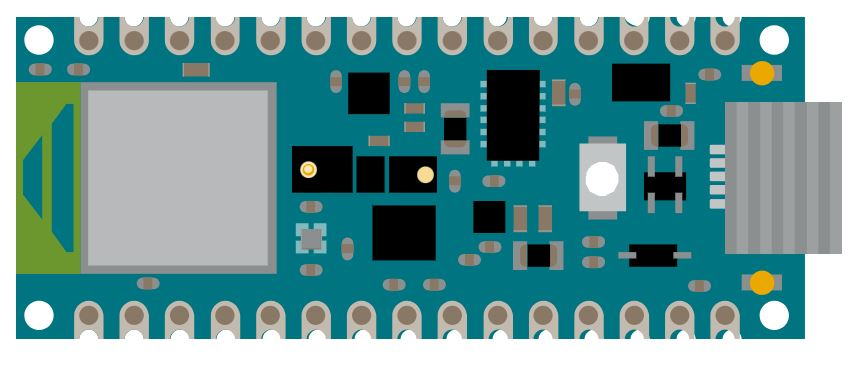
\includegraphics{Arduino/Nano33BLE/Nano33BLESense}};

  \fill[gray, opacity=0.7] (-6,-2.4) rectangle (6,2.4);

  \coordinate (A) at (\LowerLeftX,\LowerLeftY);
  \coordinate (B) at (\UpperRightX,\UpperRightY);    
  \begin{scope}
    \clip (A) rectangle (B);
    
    \node at (0,0) (Board) {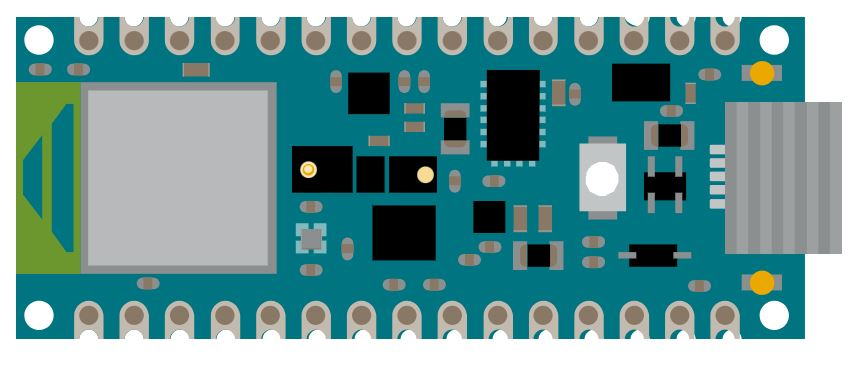
\includegraphics{Arduino/Nano33BLE/Nano33BLESense}};
    
  \end{scope}
  \draw[yellow,line width=2pt] (A)  rectangle (B);

}